\chapter{Background}

In this chapter, we will introduce the basic concepts of the Internet Protocol
Suite, briefly describe its origin, semantics, and some of its protocols.
Furthermore, SME and the hardware it will run on will be introduced as a basis
for the implementation.


\section{Internet Protocol Suite (TCP/IP)}
\begin{figure}
\centering
\includegraphics[width=\linewidth]{background/frame.eps}
\caption{Layout of a typical frame sent through the network.}
\label{fig:frame_layout}
\end{figure}


Internet Protocol Suite, better known as simply TCP/IP, is a conceptual
model providing end-to-end communication between computers. It consists of
a collection of protocols specifying the communication between multiple
Internet systems\cite{RFC1122}.  The very early research and development
on what would later become the Internet Protocol Suite began in the late 1960s
by the Defense Advanced Research Project Agency (DARPA), and was being
adopted by DARPA, as well as the public, since 1983\cite{DARPA_internet}.
Although the Internet Protocol Suite predates the newer, arguably more
refined Open Systems Interconnection (OSI) model, TCP/IP still
remains the popular choice in modern systems.  As opposed to OSI 7-layer
model\cite{X.200}, the collection of protocols in TCP/IP are organized
into 4 abstraction layers, each related to their scope of networking
involved.

\subsection{Link Layer}
\begin{figure*}
\centering
\includegraphics[scale=0.75]{background/ethernet.eps}
\caption{Layout of the Ethernet II header. The \texttt{EtherType} field is used
as \texttt{Length} in the IEEE 802.3 specification.}
\notechange[inline]{Fix line from ethertype}
\label{fig:ethernet_header}
\end{figure*}


The link layer is the lowest, bottom-most layer in the Internet Protocol Suite.
Link layer addresses methods and protocols operating on the link that the host
is physically connected to\footnote{Wireless connections are also included
under this category.}. The purpose of this layer is to send and receive IP
datagrams for the Internet Layer described in the next section.\\
Contrary to the OSI model, this lowest layer in TCP/IP
does not regard the standards and protocols of the physical mediums used
(the pin layout, voltages, cable specifications etc.), making TCP/IP
hardware-independent. As a result, TCP/IP can in theory be implemented on
virtually any hardware configuration, emphasizing the flexibility of the
model.\\
TCP/IP supports many different link layers depending on the underlying hardware
used, such as the \gls{fddi} using optical fiber cables\cite{RFC1103}, RS-232
serial lines\cite{tia_232}, or perhaps the most well-known link-layer protocol,
the Ethernet.

\subsubsection{Ethernet (II) and IEEE 802.3}
The collection of standards known under the term "Ethernet" are were originally
developed by Xerox Corp. between year 1973 and 1974\cite{americanhistory_ethernet}
\cite{tcpip_illustrated_vol1}. Version 2 of the protocol was published in 1982
under the name Ethernet II, also known as DIX Ethernet, named after 3 companies
participating in its design: DEC, Intel and Xerox\cite{heywood2001drew}.\\
Seeing wide adoption of this standard, it has been formally standardized as by
the \gls{ieee} under the publication of IEEE 802.3 in
1983\cite{ieee_8023_release}. Unfortunately, the original specification of
Ethernet frame format deviate slightly from that of IEEE
802.3\cite{tcpip_illustrated_vol1}. Figure \ref{fig:ethernet_header} shows the
layout of a standard Ethernet header. The \texttt{EtherType} field is used to
indicate the type of the payload type, whereas it is used as \texttt{Length} in
the IEEE 802.3. Fortunately, none of the valid \texttt{EtherType} values in
conventional Ethernet are valid as \texttt{Length} in the 802.3 standard, and
so the headers are easily distinguishable.\\
The divergent way of encapsulating IP datagrams is defined in RFC 894 for
true Ethernet\cite{RFC0894} and RFC 1042 for IEEE 802 networks\cite{RFC1042}.



\subsection{Internet Layer}
\begin{figure}
\includegraphics[scale=0.55]{background/ip.eps}
\caption{Layout of the IPv4 packet header}
\notechange[inline]{Fix line from TTL, Protocol, etc.}
\label{fig:ipv4_header}
\end{figure}

The internet layer mainly concerns itself with sending data from the source
network to the destination network. This seemingly simple task requires multiple
functions from the layer:
\begin{itemize}
    \item Addressing and identification
    \item Packet routing
    \item \emph{Basic} transmit diagnostic information
    \item Carrying data for various upper layer protocols
\end{itemize}

\subsubsection{Internet Protocol (IP)}
The core protocol of the Internet Layer is the aptly named Internet Protocol
(IP), which is the workhorse of the TCP/IP protocol suite.
\gls{ip} is a connectionless datagram delivery service based on the
end-to-end principle, where the application-specific computation is located on
the end nodes. It is often described as an "unreliable" protocol, as there are
no guarantees that an IP datagram successfully arrives at the intended
destination. By being connectionless, \gls{ip} does not maintain any
information about the current state about the outgoing datagrams.
As a consequence, \gls{ip} is a best effort service, in which the protocol does
its best to deliver a packet without additional knowledge of the next steps in
the network\cite{tcpip_illustrated_vol1}.\\
The first major version, and the currently most used version of the \gls{ip}
is version 4, usually referred to as \gls{ipv4}. However, it is steadily
being replaced by the newer \gls{ipv6}, with an adoption rate of over $29\%$
total users connecting to \url{www.google.com} using an IPv6 address by Jul
30, 2019\cite{google_ipv6_adoption}. Despite the improvements that the new
version provides, it has been proven to be a hard challenge to replace, update,
and modify all the existing network devices to support this new protocol,
extending the life current version 4. In this thesis, only \gls{ipv4} will
be considered.\\
\gls{ipv4} provides two basic functions: addressing and fragmentation. By using
32-bit addresses located as one of the last fields in the header on figure
\ref{fig:ipv4_header}, the nodes use the destination address to transmit
internet datagrams towards their destination. The process of selecting a path
on the network is called routing\cite{RFC0791}.\\
Fragmentation on the other hand is used to split large datagrams and transmit
these through nodes supporting smaller packets. The \texttt{Fragment Offset} in
the packet header defines the offset of the data in the datagram with the
\texttt{Identification} number.\\
\gls{ipv4} uses additional mechanisms to achieve its service:
\begin{itemize}
	\item \textbf{\gls{tos}}\\
	ToS is used to indicate the desired quality of the service provided.
	It provides options to minimize delay or monetary cost, or options to
		maximize throughput or
		reliability\cite{tcpip_illustrated_vol1}\cite{RFC0791}.
	\item \textbf{\gls{ttl}}\\
	\gls{ttl} is an upper limit of how many routers a datagram is allowed
		to pass. For every node visited, the \gls{ttl} is decremented,
		and if the counter reaches $0$, the datagram is destroyed. This
		ensures a reasonable routing by eliminating datagrams stuck in
		loops\cite{RFC0791}.
	\item \textbf{Options}\\
	Options can be added to the end of the header as a variable-list of
		optional information. It can specify additional functionality
		during the transmission, such as timestamping, routing options,
		security restrictions etc.. However, since it is not required
		to support Options in the \gls{ipv4} header, these are rarely
		supported and used\cite{tcpip_illustrated_vol1}.
	\item \textbf{Header Checksum}\\
	To ensure the correct routing and handling of the IP datagram, the
		checksum in the header assures the header-part of the packet is
		intact. Note that the checksum is only calculated for the
		header, and not the data, as this is done by most transport
		protocols.
\end{itemize}


\subsection{Transport Layer}
The transport layer establishes end-to-end data transfer between hosts.
Protocols in the transport layer can provide additional services to the user,
such as reliability, ordering, error- and flow-control, application addressing
(port numbers), error-checking, and so on.\\
While it is possible to bypass the protocols in this layer on most modern
network stacks, the protocols in the transport layer provide such essential
and useful services that it hardly ever makes sense to implement in the
application layer.

\subsubsection{Transmission Control Protocol}
\begin{figure}
\includegraphics[scale=0.55]{background/tcp.eps}
\caption{Layout of the TCP packet header}
\label{fig:tcp_header}
\end{figure}

While there are numerous protocols defined in the Transport Layer, perhaps the
most well-known protocol in the stack is the \gls{tcp}.
Being one of the most used transport protocol for its reliability and congestion
control systems, it is rightly justified to refer to the whole Internet Protocol
Suite as simply "TCP/IP".

Since \gls{tcp} prioritizes reliability of transmission rather than timely
delivery, it is extensively used in applications which require these
properties. For instance, this protocol is essential in key internet applications
 such as the \gls{ftp}, \gls{ssh} and \gls{www}.


\subsubsection{User Datagram Protocol}
\begin{figure}
\includegraphics[scale=0.55]{background/udp.eps}
\caption{Layout of the UDP packet header}
\label{fig:udp_header}
\end{figure}

The \gls{udp} is a stark opposite to \gls{tcp}, as it is connectionless and
unreliable in the sense that a sent segment might never arrive.
Additionally, there is no handshake process, and the segments might arrive in
a different order than they have been sent.

However, by removing all these features, \gls{udp} has a lot less overhead. The
only thing the protocol needs to have is the source and destination port, the
length of the data, and the checksum thereof, illustrated on figure
\ref{fig:udp_header}. This simple nature of the protocol makes it possible to
be very fast and responsive, and it has found its utility in \gls{voip},
\gls{p2p} file-transfer, as well as online multiplayer games.

\subsection{Application Layer}
The application layer protocols are used by applications and services to
exchange information over the network. A few of the well-known application
layer protocols are the \gls{http}\cite{RFC1945},
\gls{ftp}\cite{RFC0114}, and \gls{smtp}\cite{RFC0788}.\\
This layer is usually implemented by the user-space applications themselves, and
therefore are not strictly required to actually run a TCP/IP network.



\section{Hardware}
The networking stack is intended to be flexible enough to run on just about any
configuration of hardware and software. However, this also means that it cannot
depend on any major external components, such as an existing memory, a processor,
or any form of operating system. Fundamentally, not only the software-part of the
networking stack has to be implemented, but the hardware needs to be defined
as well. This hardware should be self-contained enough to work well in combination
with any additional system, which the user incorporate for networking.\\
A wide variety of hardware types exist for such independent system, such as
\gls{asic}, \gls{cpld}, \gls{soc}, and \gls{fpga}.
\notecarl{Mark: SoC referer til et helt system, f.eks. et board, ikke en chip. En SoC har oftest en ASIC eller en FPGA. Senere refererer i til Zynq, som ganske rigtigt kan betragtes som en SoC, fordi den både har en ARM processor, en FPGA osv.}
Each of these integrated circuits have their advantages and disadvantages; some
of them are re-programmable, some are cheap and disposable, and some are excellent
for general-purpose applications.\\


\subsection{Field Programmable Gate Array (FPGA)}
Field Programmable Gate Arrays, or FPGA for short, are devices containing
integrated circuits (ICs) consisting of arrays of logic blocks.
These logic blocks can be programmed to form arbitrary logic circuit by simply
synthesizing a design and then loading it onto the board. This process alone
can save the manufacturer months by not having to fabricate a whole new IC. \\
FPGAs can be used for any computational tasks without the need of any additional
hardware. Usually, these devices are used for smaller, domain-specific tasks,
where the control over the hardware yields significant performance increases.
FPGAs are indeed very universal, and can be used in product-design, prototyping,
as well as in final products. Products like car driver assistance
systems\cite{xilinx_fpga_automotive}, audio decoders\cite{xilinx_fpga_audio},
or even internet search engines\cite{bing_search_fpga}  all utilize FPGAs to
increase the performance, lower the electrical bill, and  boost the development
potential.

\subsubsection{Technical specifications}
Field Programmable Gate Arrays consists of a vast number of ICs, which can
be reprogrammed at any time for a desired application or functionality\cite{ni_fpga},
making the devices very flexible and extensible, even after manufacturing.\\
These ICs are practically totally independent, and their logic within can be
programmed and combined in virtually any way with other ICs. This, however,
poses a problem, as signals do not propagate through circuitry, immediately, but
rather, they have a slight delay.
Sometimes, two events precede each other, while other times, events of distinct
timings must occur simultaneously.
Since the order of events is critical for correct and expected execution in
digital circuits, a digital clock is used to ensure everything runs in sync.
A clock in this context emits a series of pulses in a pre-determined and very
precise interval. These pulses are used to control the execution of various
elements in the circuitry.\\
When synthesizing to a FPGA, the compiler finds the longest code-path, it finds
the required circuitry to perform the calculation, and then it determines the
minimal required time for the signals to propagate through the path. In this
manner, the fastest possible clock can be found for that particular circuit.\footnote{
    Although many modern FPGAs consist of multiple regions which can have individual
    clock-rates. While it is a demanding task to propagate signals across these
    boundaries, a performance increases can be gained.
}
With innovations and steady improvements in modern FPGAs, the circuitries within
the devices can be clocked at higher than 500 MHz\cite{xilinx_fpga}.


\subsection{Application-specific integrated circuit (ASIC)}
\gls{asic} is an integrated circuit consisting of components such as
transistors, capacitors, and resistors. During the manufacturing of an
\gls{asic}, the electrical design with the intended functionality is hardwired
onto the board. This enables the devices to be very compact, efficient, fast,
and low-power. Unfortunately, with this permanent nature of the board, the
functionality cannot be changed after the fabrication, and the board has to be
replaced in order to introduce new functionality\cite{fpga_for_dummies}.\\
The immutability of \gls{asic} boards make them very inefficient for
prototyping, but the bulk production once the final design is found can drive
the per-device price down significantly. However, it is to be noted that
some businesses still chose \gls{fpga} in finalized products in order to be
able to patch and update the devices after the release, avoiding costly
replacements if problems are found after the fact.\cite{fpga_for_dummies}


\subsection{Complex Programmable Logic Devices (CPLD)}
\gls{cpld} are consists of a fully programmable AND/OR gate array and a set of
macrocells. Macrocells are units prefabricated with higher-level functionality,
such as \gls{alu}s, registers, and flip-flops. Since these macrocells are
pre-made by the manufacturer, they can be heavily optimized in regards to both
performance, but also power efficiency.\cite{xilinx_cpld}\\
\gls{cpld} devices are re-programmable, but unlike \gls{fpga}s
\notecarl{Mark:  Side note: man laver også boards med FPGA, hvor deres bitstream er gemt i en ROM, så de heller ikke kan blive reflashet. Eller rettere sagt, en FPGA kan kun blive reflashet, hvis man designer boardet til at kunne det. Men generelt har i ret!}
, \gls{cpld} are
non-volatile since their programming is stored on \gls{eeprom}. This means that
the programming is kept on power down, and the functionality is active as soon
as the device is turned on\cite{xilinx_cpld}.\\
Unfortunately, with the introduction of the pre-made functionality in the
macrocells, a bit of flexibility and extensibility is lost compared to
\gls{fpga}. For instance, while it is easy to integrate \gls{fpga} with
external memory chips, \gls{cpld} has no on-die dedicated hardware (IP)
available for offloading\cite{numatolab_cpld_vs_fpga}.

\subsection{Choosing \gls{fpga} for prototyping}
In this thesis, only FPGAs will be taken into consideration for
its re-programmability, its fairly low-cost, availability, and the
compatibility with SME code-generators. During the implementation, the
TUL PYNQ\texttrademark-Z2 FPGA board will be used for prototyping. This
board is based on Xilinx Zynq \gls{soc}, and is an excellent device
for smaller projects given its wide assortment of documentation to get
started prototyping.\cite{tul_pynq}





\subsubsection{Programming an FPGA}
Unlike conventional processors with a very sequential nature, the logic blocks
in FPGAs are truly parallel in nature. Given the right programming, an FPGA can
allocate \notecarl{Mark: Pas på her, fordi det er ikke allokering i samme sense som f.eks. med memory allokering. Man kan godt allokere en FPGA runtime, men det er ikke på helt samme måde som man gør ved synthesis. I det tilfælde bliver FPGA'en basically lavet om til en GPU, hvor man bruger meget af FPGA'en til at manage hvad der kører hvor. Ellers kan man også lave partial reconfiguration, men det er uden for jeres scope!}
dedicated sections of the chip for each independent subtask, enabling
the circuitry to perform numerous independent calculations at once\cite{ni_fpga}.
Unfortunately, this universality of FPGAs comes at a cost to their performance.
Whereas conventional processors are heavily optimise based on the predetermined
circuitry, FPGAs programmers must ensure to utilize the parallel nature of the
device in order to secure best possible performance.
\notecarl{Mark: Skal en CPU og GPU dog også}
Even worse, the FPGA must
be programmed in such a way that all paths in the electrical wiring can be
in any time-frame.\\
Due to this parallel nature of FPGAs, conventional programming languages are
next to impossible to use. To define the behavior of an FPGA, Hardware
Description Languages (HDL) are used. These programming languages are not easy
to learn without a good grasp of electrical engineering. Even with prior
programming knowledge, the unusual approach to concurrency in these languages
can be hard to understand for average developers.\\
To simplify the development process, most manufacturers offer predefined
circuits along their FPGAs. These predefined circuits are more commonly known
as Intellectual Property (IP) cores, and can provide the hardware designers
with pre-made circuitry for a wide variety of functionality. While most IPs
provide the functionality of processors for testing
\notecarl{Source?}
on an FPGA, mp3 audio
decoding or PCI bus interconnect can be obtained as well\cite{fpga_for_dummies}.



\section{Synchronous Message Exchange}
The Synchronous Message Exchange
model (SME) is a messaging framework created in order to help model
hardware descriptions\cite{sme_for_hardware_designs}.  It was conceived
once the flaws of using Communicating Sequential Processes (CSP) was
identified during the modelling of a vector processor with CSP using
PyCSP\cite{PyCSP}.  It turned out that there is a major discrepancy
between the way data is propagated in hardware opposed to that of the
CSP model. While CSP does not pose any requirements on the communication
between processes, in digital hardware, all communication has to be
synchronized, driven by a clock. To combat this in the CSP model, a
global clock process needed to be implemented, which was connected to
all other processes. Additionally, latches had to be introduced in order
to not overwrite values during a cycle. This caused an explosion of both
channels and latches in the final design, making CSP a much less viable
framework for hardware modelling\cite{sme_for_hardware_designs}.

\subsection{The model} The SME model consists of only a few fundamental
concepts. Each SME model is a \textit{network} consisting of one or more
\textit{processes}. These processes do not share any memory or storage,
but are interconnected with \textit{busses}.  These busses are perhaps
the most interesting units in SME model, as they not only propagate
information between processes using the underlying \textit{channels},
but also introduce an implicit clock between the processes.\\

\subsection{Process execution flow}
The default execution flow of a process is
fairly simple, and relates very closely to that of the actual hardware. At
the beginning of a clock-cycle, the input-ports are read into the busses
they are connected to. Then, the process executes its "compute" stage, and
the results, if any, are written to the output-port, which will be read
by the following bus. A visualization of the execution flow can be seen
on figure \ref{fig:sme_clock}.
\pic{0.5}{background/sme_clock}{An illustration of a typical SME clock-cycle}{fig:sme_clock}
It is important to note that although certain channels might be written earlier
than others in a process clock, the subsequent processes connected to said bus
will first see the values change in the beginning of the next clock
cycle.

However, it is important to note that in the newer \gls{sme} model, the network
supports clock-multipliers. In certain situations, it is desirable to clock the
processes faster than the parent network. Here, \gls{sme} will clock the
network at an integer multiplier of the parent network.

\subsection{Using SME}
SME has undergone multiple iterations, reworks, and extensions. While
it is still under very active testing and development, its core
functionalities and features
 are well-established and stable\cite{bus_centric_sme}.\\
SME has concurrent implementations in the C\# and Python languages,
with promising efforts to unify these under a common intermediate
domain-specific language SMEIL\cite{smeil}. The C\# version has
exhibited various advantages over the Python counterpart, such as
the more error-prone strong typing system, which better reflects the
functionality of the hardware, as well as making the code more readable to
the programmer. At the time of writing, the C\# implementation currently
enjoys the most recent features of the SME model, as it is being the
most actively developed version.


